\documentclass[tikz,border=1pt]{standalone}
\usetikzlibrary{shapes.geometric, arrows.meta, positioning, fit, backgrounds}
\begin{document}
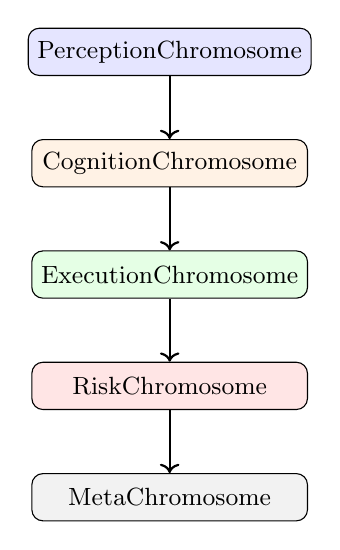
\begin{tikzpicture}[node distance=0.8cm,
    chrom/.style={draw, rectangle, rounded corners, minimum width=3.5cm, minimum height=0.6cm, align=center, font=\small}]
    \node[chrom, fill=blue!10] (p1) {PerceptionChromosome};
    \node[chrom, below=of p1, fill=orange!10] (p2) {CognitionChromosome};
    \node[chrom, below=of p2, fill=green!10] (p3) {ExecutionChromosome};
    \node[chrom, below=of p3, fill=red!10] (p4) {RiskChromosome};
    \node[chrom, below=of p4, fill=gray!10] (p5) {MetaChromosome};
    \draw[->, thick] (p1) -- (p2);
    \draw[->, thick] (p2) -- (p3);
    \draw[->, thick] (p3) -- (p4);
    \draw[->, thick] (p4) -- (p5);
\end{tikzpicture}
\end{document}
